\documentclass[compress]{beamer}
\usepackage{ifthen,verbatim}

\title{New Muon System Alignment Procedure \\ and the Effect of Residual Misalignments \\ on TeV-scale muons}
\author{Jim Pivarski, Alexei Safonov}
\institute{Texas A\&M University}
\date{11 December, 2007}

\newcommand{\isnote}{}
\xdefinecolor{lightyellow}{rgb}{1.,1.,0.25}
\xdefinecolor{darkblue}{rgb}{0.1,0.1,0.7}
\xdefinecolor{darkgreen}{rgb}{0.,0.5,0.}
\xdefinecolor{greyone}{rgb}{0.6,0.6,0.6}
\xdefinecolor{greytwo}{rgb}{0.4,0.4,0.4}
\xdefinecolor{greythree}{rgb}{0.2,0.2,0.2}
\xdefinecolor{greyfour}{rgb}{0.1,0.1,0.1}

%% Uncomment this to get annotations
%% \def\notes{\addtocounter{page}{-1}
%%            \renewcommand{\isnote}{*}
%% 	   \beamertemplateshadingbackground{lightyellow}{white}
%%            \begin{frame}
%%            \frametitle{Notes for the previous page (page \insertpagenumber)}
%%            \itemize}
%% \def\endnotes{\enditemize
%% 	      \end{frame}
%%               \beamertemplateshadingbackground{white}{white}
%%               \renewcommand{\isnote}{}}

%% Uncomment this to not get annotations
\def\notes{\comment}
\def\endnotes{\endcomment}

\setbeamertemplate{navigation symbols}{}
\setbeamertemplate{headline}{\includegraphics[height=1 cm]{../cmslogo} \hspace{0.1 cm} \includegraphics[height=1 cm]{../tamulogo} \hfill
\begin{minipage}{5.5 cm}
\vspace{-0.75 cm} \small
\begin{center}
\ifthenelse{\equal{\insertpagenumber}{1}}{}{\textcolor{blue}{\insertsection}}
\end{center}
\end{minipage} \hfill
\begin{minipage}{4.5 cm}
\vspace{-0.75 cm} \small
\begin{flushright}
\ifthenelse{\equal{\insertpagenumber}{1}}{}{Jim Pivarski \hspace{0.5 cm} \insertpagenumber\isnote/\pageref{numpages}}
\end{flushright}
\end{minipage}\mbox{\hspace{0.2 cm}}}

\begin{document}
\frame{\titlepage}

%% \begin{notes}
%% \item This is the annotated version of my talk.
%% \item If you want the version that I am presenting, download the one
%% labeled ``slides'' on Indico (or just ignore these yellow pages).
%% \item The annotated version is provided for extra detail and a written
%% record of comments that I intend to make orally.
%% \item Yellow notes refer to the content on the {\it previous} page.
%% \item All other slides are identical for the two versions.
%% \end{notes}

%% 1. why we need a new procedure (reminder about the bug that made old results too optimistic)
%% 2. key issue in muon alignment; how we can address this in the current framework
%% 3. results from the new procedure: accuracy of aligned positions and resolution of TeV muons
%% 4. general studies of TeV muon resolution, comparison with official scenarios
%% 5. what's going into the TeVmu note

\begin{frame}
\frametitle{Overview}
\begin{itemize}\setlength{\itemsep}{0.75 cm}
\item Lessons learned from CSA07
\item New alignment procedure developed as a response
\item New alignment results
\item Effect of misalignments on TeV muons
\end{itemize}
\end{frame}

\section*{Lessons from CSA07}

\begin{frame}
\begin{center}
\Huge \textcolor{darkblue}{Lessons from CSA07}
\end{center}
\end{frame}

\begin{frame}
\frametitle{Story since our last meeting}

\begin{itemize}\setlength{\itemsep}{0.25 cm}
\item CSA07 exercise was just like our private tests, {\it except}
that misalignment was applied during original track fits
\item Should be irrelevant, because misalignment is reapplied (replaced)
during track refits, every iteration
\item But this difference unveiled a mistake in our procedure which
made our old results too optimistic (next slide)
\item We corrected the mistake
\item Retuned the procedure
\item Repeated the 10~pb$^{-1}$ exercise
\item Results from this exercise and effect on TeV muons in this talk
\end{itemize}
\end{frame}

\begin{frame}
\frametitle{What was wrong in the old procedure?}
\begin{columns}
\column{0.55\linewidth}
\begin{itemize}\setlength{\itemsep}{0.2 cm}
\item Tracks were refit from the outermost radius, inward
\item The refit algorithm was told to de-weight muon hits (because
their exact locations are not well known before alignment)
\item Resulting track is mostly unmodified in the
muon system, especially at large radius
\end{itemize}
\column{0.5\linewidth}
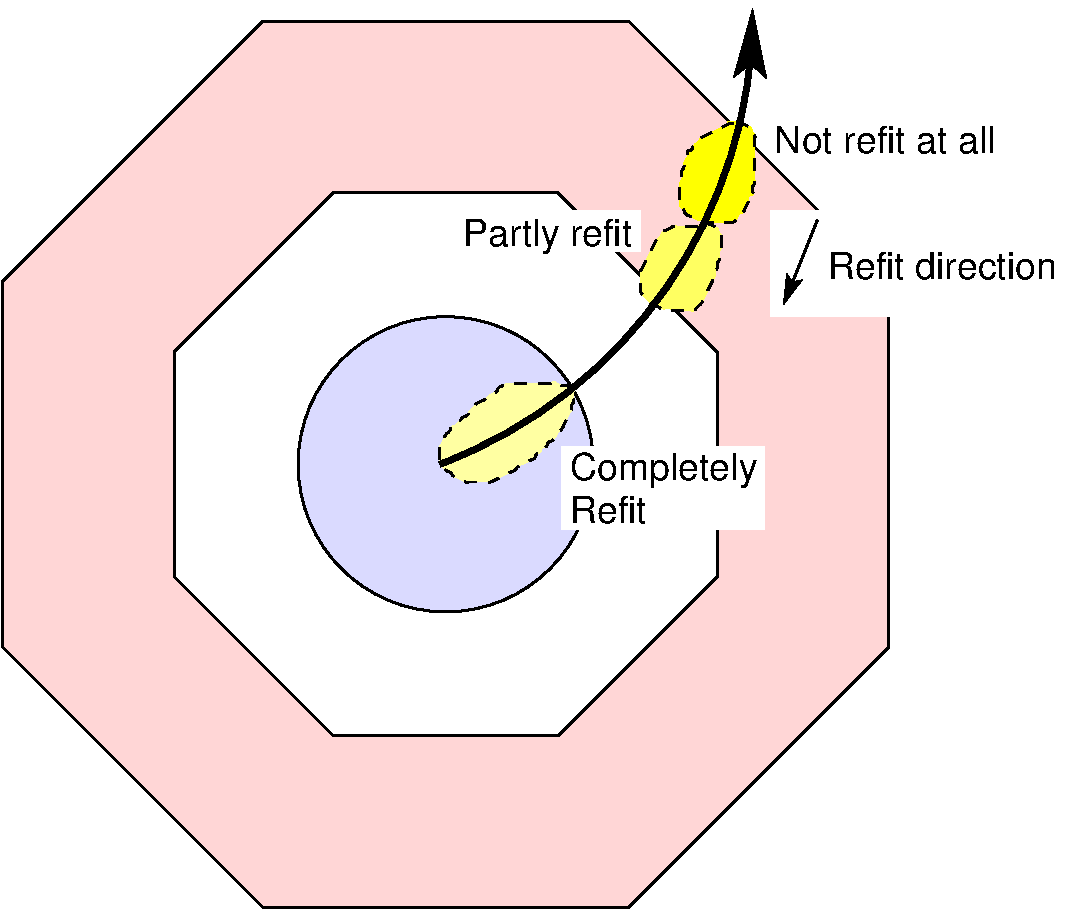
\includegraphics[width=\linewidth]{whatwaswrong.pdf}
\end{columns}

\vspace{0.3 cm}
\mbox{ }

\hspace{-0.5 cm}\begin{minipage}{\linewidth}
\begin{itemize}\setlength{\itemsep}{0.2 cm}
\item This yields too-optimistic alignment results because the
unmodified part of the track ``remembers'' the alignment used in the
original track fit (usually ideal, but not in CSA07)
\item Solution: fit outward to extrapolate from tracker, as intended
\end{itemize}
\end{minipage}
\end{frame}

\begin{frame}
\frametitle{What does this affect?}
\begin{itemize}\setlength{\itemsep}{0.5 cm}
\item Our alignment results presented before November need
to be replaced, including systematics studies
\item We should re-address questions such as whether to prefer a high
momentum cut or large statistics
\item CPU requirements will be larger (people in charge of the CAF have been notified)
\item With proper track extrapolations, we find that scattering
in material is more significant than we previously thought: \\ we'll
need special techniques to minimize extrapolation
\end{itemize}
\end{frame}

\section*{The new procedure and first results}

\begin{frame}
\begin{center}
\Huge \textcolor{darkblue}{The new procedure and \\ first results}
\end{center}
\end{frame}

\begin{frame}
\frametitle{Track propagation through material}
\begin{columns}
\column{0.7\linewidth}
\begin{itemize}\setlength{\itemsep}{0.25 cm}
\item Real muons can change direction in the
iron/solenoid/calorimeter, leading to changes in trajectory of
$\mathcal{O}(\mbox{cm})$
\item The track-fitter knows this and compensates
\item With small Alignment Parameter Errors (APEs), misalignments are
absorbed into scattering; resulting track is useless for alignment
\item With large APEs, residuals are huge; alignment is imprecise
\item \mbox{Minimizing track extrapolation helps a lot \hspace{-1 cm}}
\end{itemize}
\column{0.3\linewidth}
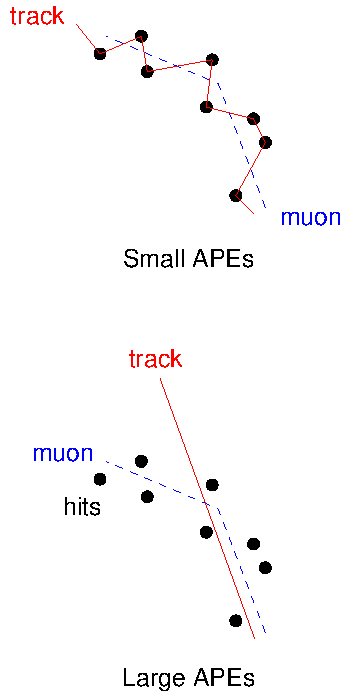
\includegraphics[width=\linewidth]{flexibility.pdf}
\end{columns}
\end{frame}

\begin{frame}
\frametitle{Aligning in passes}

\begin{itemize}\setlength{\itemsep}{0.25 cm}
\item One way to minimize extrapolation is to align stations
sequentially, propagating tracks only from previous station
\item For example, to align station 2
\begin{enumerate}\setlength{\itemsep}{0.1 cm}
\item Guarantee that station 1 is fully aligned
\item Fit tracks with APE = 0 in station 1, APE = medium in station 2, and APE = large in stations 3 onward
\item Align station 2 to residuals
\end{enumerate}

\item \textcolor{darkblue}{Pro:} smaller extrapolation length without new code

\item \textcolor{darkblue}{Con:} CPU intensive (same tracks are refit many times)
\end{itemize}

\vspace{0.3 cm}
\hspace{-0.83 cm} \textcolor{darkblue}{\Large Alternative}

\begin{itemize}
\item Change track-fitter, e.g.\ alignment from overlaps
\end{itemize}
\end{frame}

\begin{frame}
\frametitle{9-pass procedure}
\begin{columns}
\column{0.45\linewidth}
\scriptsize
\begin{enumerate}\setlength{\itemsep}{0.05 cm}
\item Align wheels and disks
\item Pass 1: align MB1 and ME1/1
\item Pass 2: align MB2 and ME1/2
\item Pass 3: align MB3 and ME2/1
\item Pass 4: align MB4 and ME1/3
\item Pass 5: align ME2/2 and ME3/1
\item Pass 6: align ME3/2 and ME4/1
\item ``Stage 3'': re-align everything with 500~$\mu$m APEs
\item ``Stage 4'': re-align everything but MB1, ME1/1, and ME1/2
\end{enumerate}
\column{0.6\linewidth}
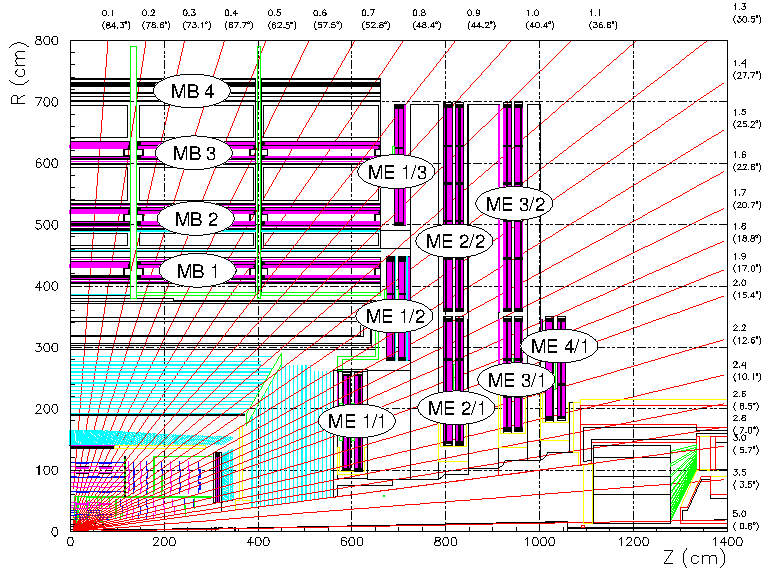
\includegraphics[width=\linewidth]{muon_system_labeled.pdf}
\end{columns}

\vspace{0.2 cm}
\begin{itemize}\setlength{\itemsep}{0.1 cm}
\item Stations aligned simultaneously don't share any tracks
\item APEs independently optimized for each stage
\item Stage 3 makes sure we don't end with relative alignments only
\item Stage 4 makes sure we still have relative alignments
\end{itemize}
\end{frame}

\begin{frame}
\frametitle{First results: test for alignment quality}

\begin{itemize}\setlength{\itemsep}{0.1 cm}
\item Using 66,000 muons from 10~pb$^{-1}$ of $W$ decays \\ (adding the 5,400 muons from $Z$ can only help)
\item Starting with complete misalignment: $\pm$5~mm, $\pm$5~mrad at all levels (chamber and wheel/disk)
\item Includes known layer misalignments in CSCs (which we won't improve with this procedure)
\item Two cases:
\begin{itemize}
\item Ideal tracker
\item 10~pb$^{-1}$ misaligned tracker
\end{itemize}
\item Two methods to judge quality:
\begin{itemize}
\item Dimuon resolution for 3.5~TeV Z' (where muon alignment matters most)
\item Stdev of local $x$ (global $r\phi$) residual misalignment, for each station
\end{itemize}
\end{itemize}
\end{frame}

\begin{frame}
\frametitle{\only<1>{Ideal}\only<2>{Misaligned} tracker case}
Dashed line: perfect muon system alignment (best-case goal)

Grey line: official 10 pb$^{-1}$ scenario (not a mean)

\vfill
\only<1>{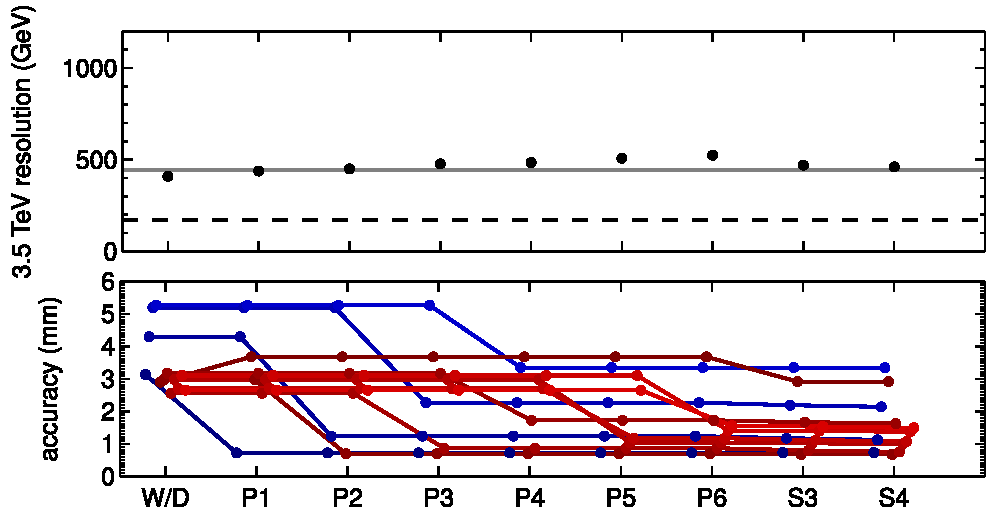
\includegraphics[width=\linewidth]{ideal_tracker.pdf}}\only<2>{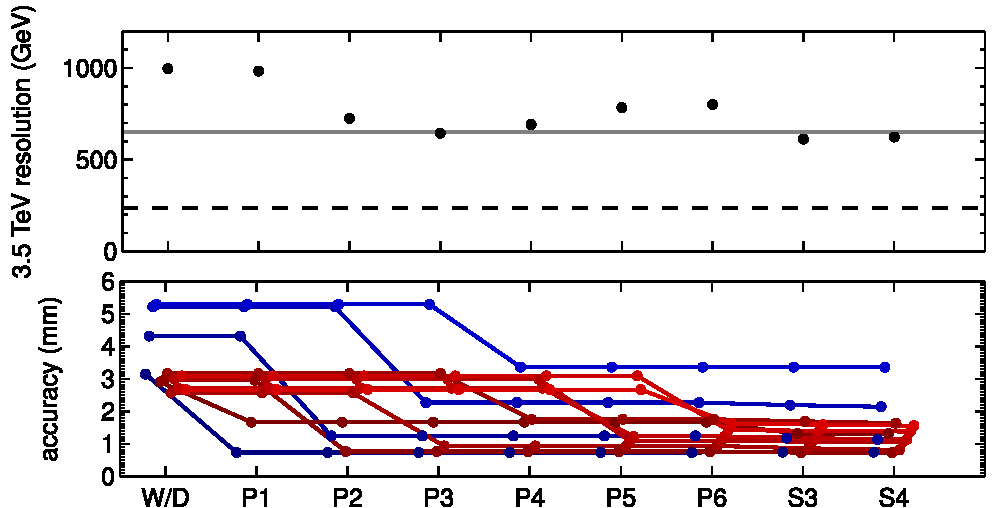
\includegraphics[width=\linewidth]{misaligned_tracker.pdf}}

\vfill
\textcolor{red}{Reds:} endcap stations, \textcolor{blue}{Blues:} barrel stations
\end{frame}

\begin{frame}
\frametitle{Shown as a raw dimuon spectrum (\only<1>{ideal}\only<2>{misaligned} tracker case)}
\begin{center}
\only<1>{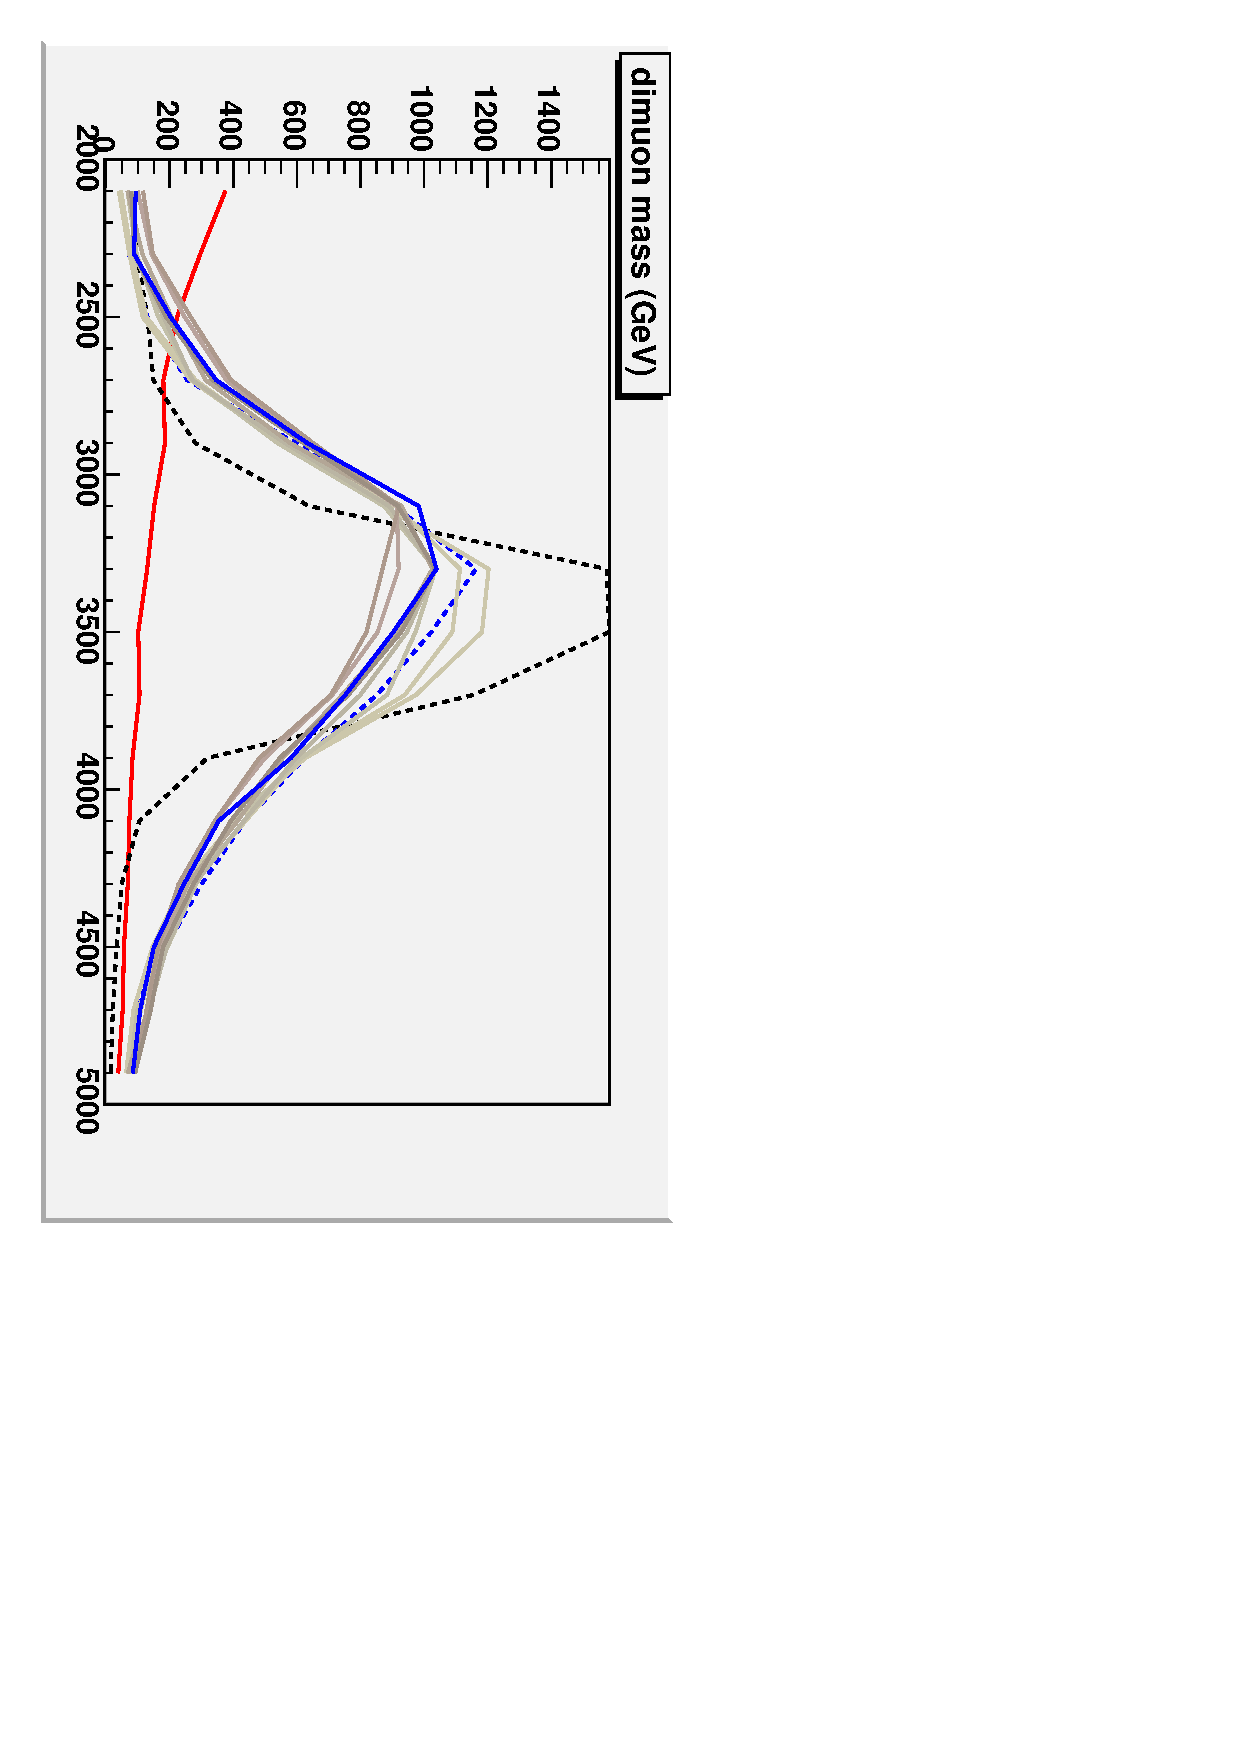
\includegraphics[height=0.8\linewidth, angle=90]{all_superimposed_ideal.pdf}}\only<2>{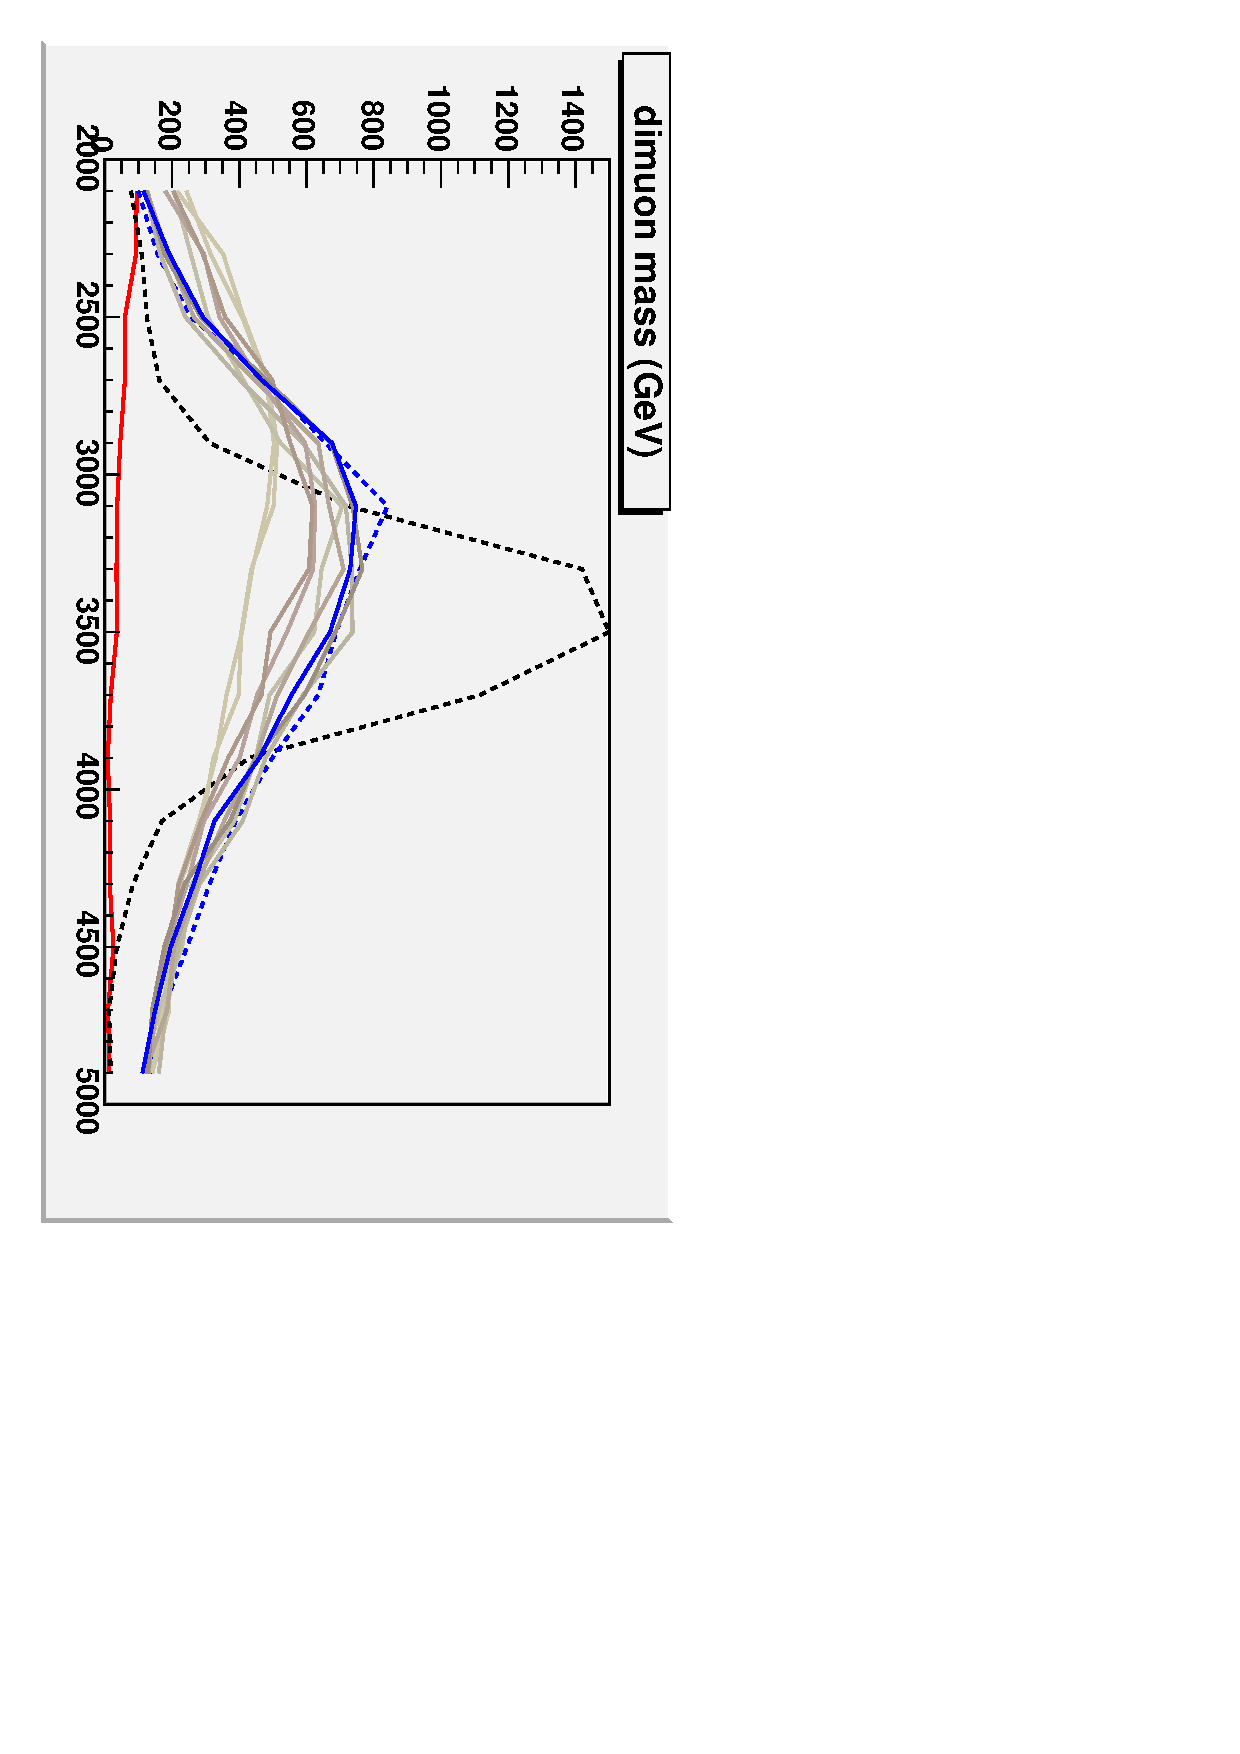
\includegraphics[height=0.8\linewidth, angle=90]{all_superimposed.pdf}}
\end{center}

\vfill \textcolor{red}{Red:} before alignment (peaks at 1~TeV)

\textcolor{greyone}{Darkening} \textcolor{greytwo}{shades} \textcolor{greythree}{of} \textcolor{greyfour}{gray:} alignment passes, ending in \textcolor{blue}{blue}

\textcolor{blue}{Dashed blue:} official 10~pb$^{-1}$ scenario

Dashed black: perfect muon system alignment
\end{frame}





\section*{TeV muon resolution}

\begin{frame}
\begin{center}
\Huge \textcolor{darkblue}{General studies of \\ TeV muon resolution}
\end{center}
\end{frame}

\begin{frame}
\frametitle{State of the ``official'' muon misalignment scenarios}
\begin{itemize}\setlength{\itemsep}{0.3 cm}
\item 10 and 100 pb$^{-1}$ muon misalignment scenarios in the database were generated
under different assumptions

\vspace{0.1 cm}
\begin{center}
\scriptsize
\renewcommand{\arraystretch}{1.25}
\begin{tabular}{c | c}
10 pb$^{-1}$ (short-term) & 100 pb$^{-1}$ (long-term) \\\hline
0.5 mm chamber misalignments & 0.2 mm chamber misalignments \\
\textcolor{darkgreen}{2 mm wheel/disk misalignments} & \textcolor{blue}{1 mm sector misalignments} \\
& \textcolor{red}{1 mm whole muon system misalignment} \\
\end{tabular}
\end{center}

\vspace{0. cm}
\item Misalignment of largest structures dominate TeV muon resolution
\item 100 pb$^{-1}$ scenario depends strongly on random number seed
\item 10 and 100 pb$^{-1}$ scenarios in the database have nearly equal
TeV muon resolutions (100 pb$^{-1}$ is slightly worse; it fluctuated up)
\end{itemize}
\end{frame}

%% \item Largest structures matter most for dimuon resolution, 
%% \begin{center}
%% 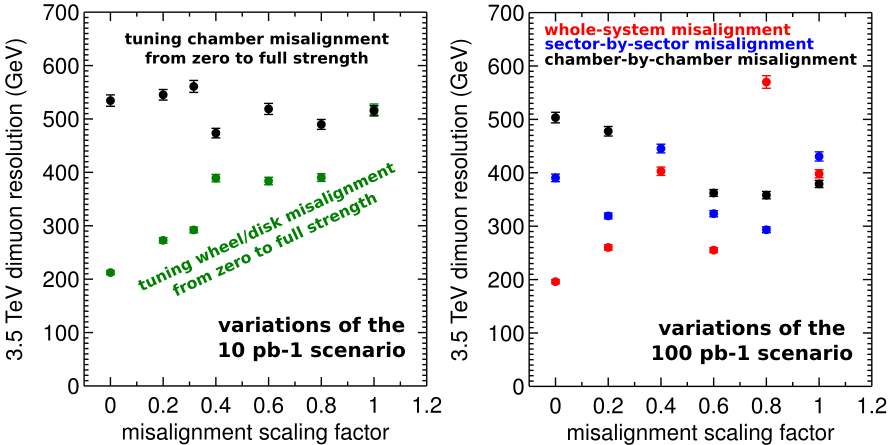
\includegraphics[width=0.8\linewidth]{scaling_misalignments.png}
%% \end{center}
%% \end{itemize}

\begin{frame}
\frametitle{Misalignment scenario from new alignment procedure}
\begin{itemize}\setlength{\itemsep}{0.25 cm}
\item More realistic because
\begin{itemize}\setlength{\itemsep}{0.1 cm}
\item errors derived directly from measurements (including $\sigma_x \ne \sigma_y$)
\item correlations along line of sight of tracks are implicitly included
\item as well as all other detector effects modeled by the Monte Carlo
\end{itemize}

\item Still conservative because
\begin{itemize}\setlength{\itemsep}{0.1 cm}
\item procedure has not been fully optimized yet, nor does it include input from hardware alignment system
\item adding muons from $Z$ will help, low-$p_T$ muons may help
\item assumes CSC layer misalignment is not improved
\end{itemize}

\item Currently, only the 10 pb$^{-1}$ results are available: included as a
place-holder in the following plots
\item Will be replaced by 100~pb$^{-1}$ results in 2 weeks
\end{itemize}
\end{frame}

\begin{frame}
\frametitle{Effect on resonance peak (${Z'}_{SSM}$ from 1 to 3.5 TeV)}

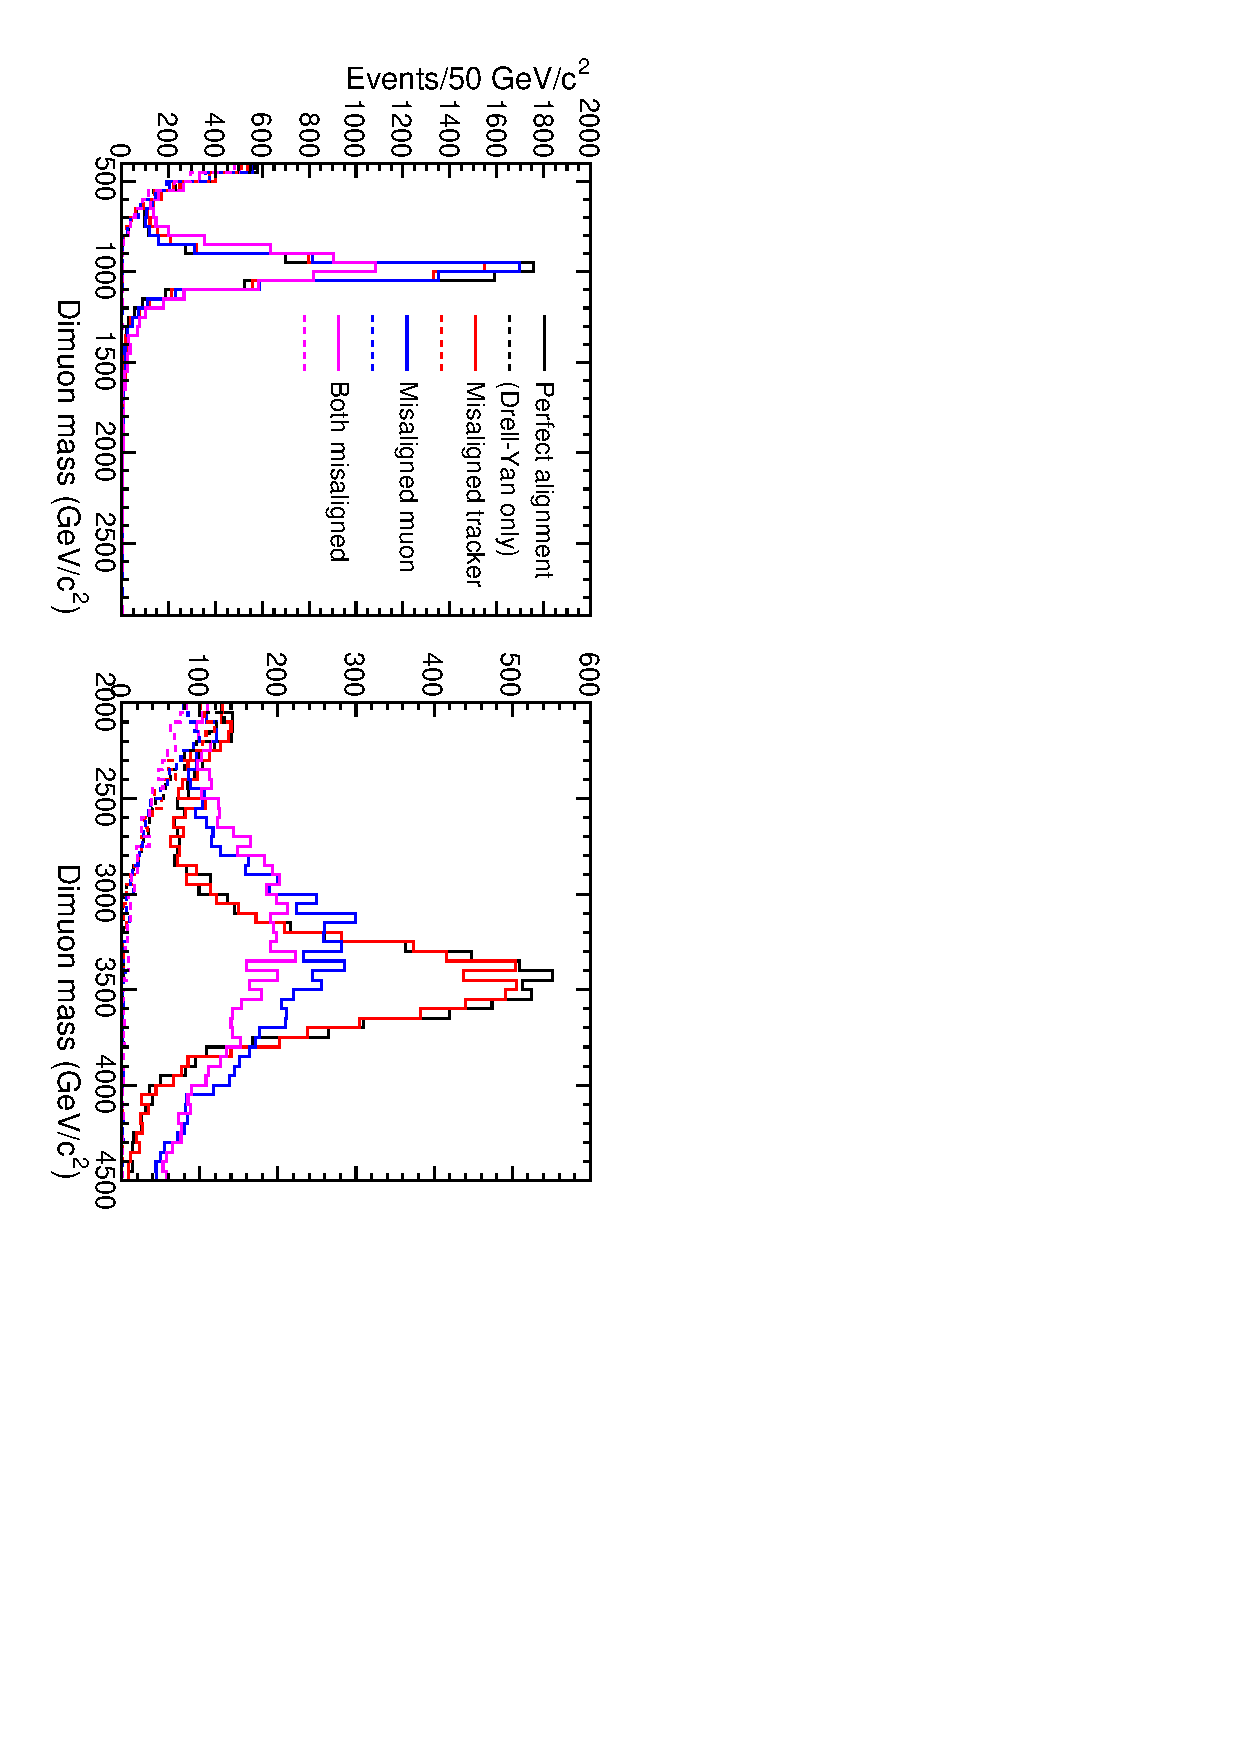
\includegraphics[height=\linewidth, angle=90]{ZSSM_Align_Spectra_1_35_TeV.pdf}

\begin{itemize}
\item ``Misaligned muon'' is from the realistic alignment procedure, but results are similar to official scenarios
\item Drell-Yan background doesn't spread up, but peak shifts down
\end{itemize}
\end{frame}

\begin{frame}
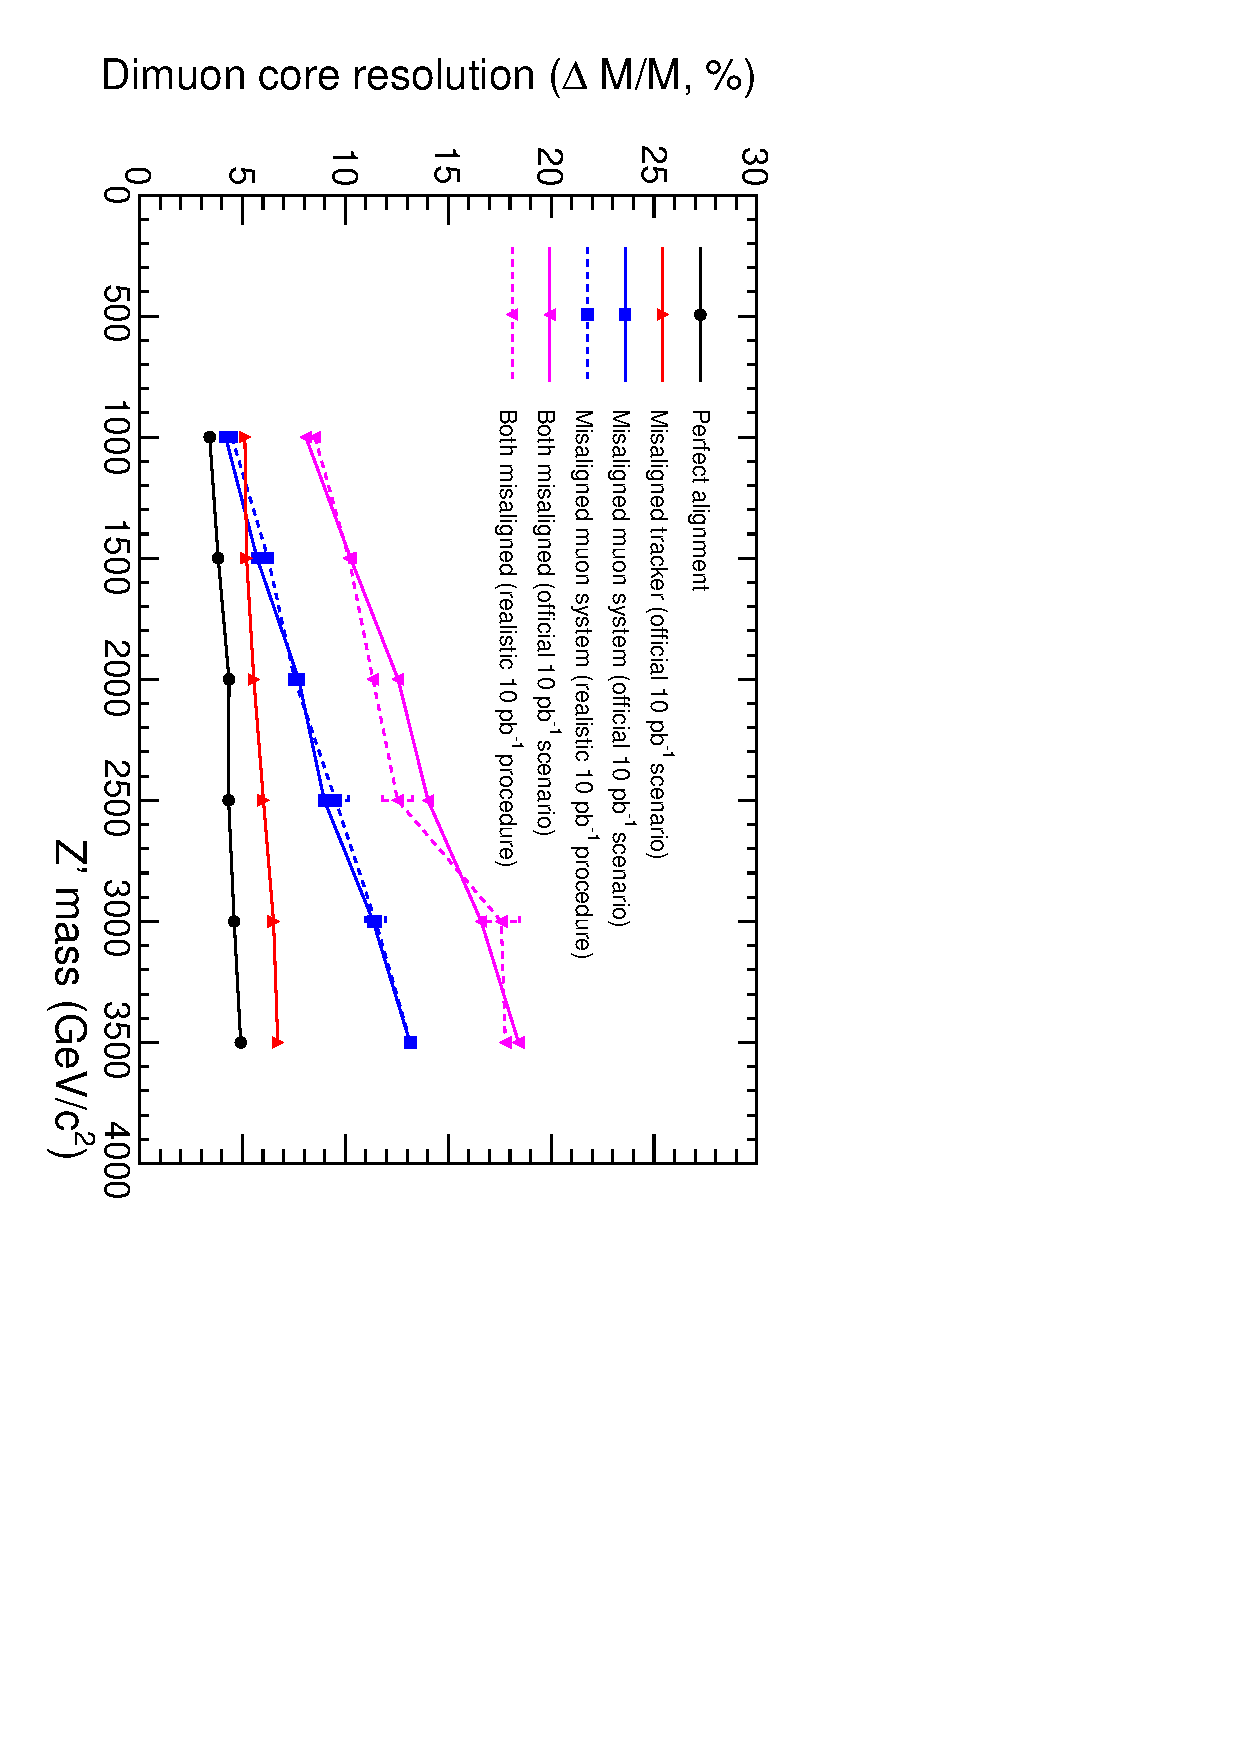
\includegraphics[height=\linewidth, angle=90]{ZSSM_Align_MassRes_color.pdf}
\begin{itemize}
\item ``Core resolution'' from a fit to each $\displaystyle \frac{\Delta M}{M}$ peak (ignores tails)
\end{itemize}
\end{frame}

\begin{frame}
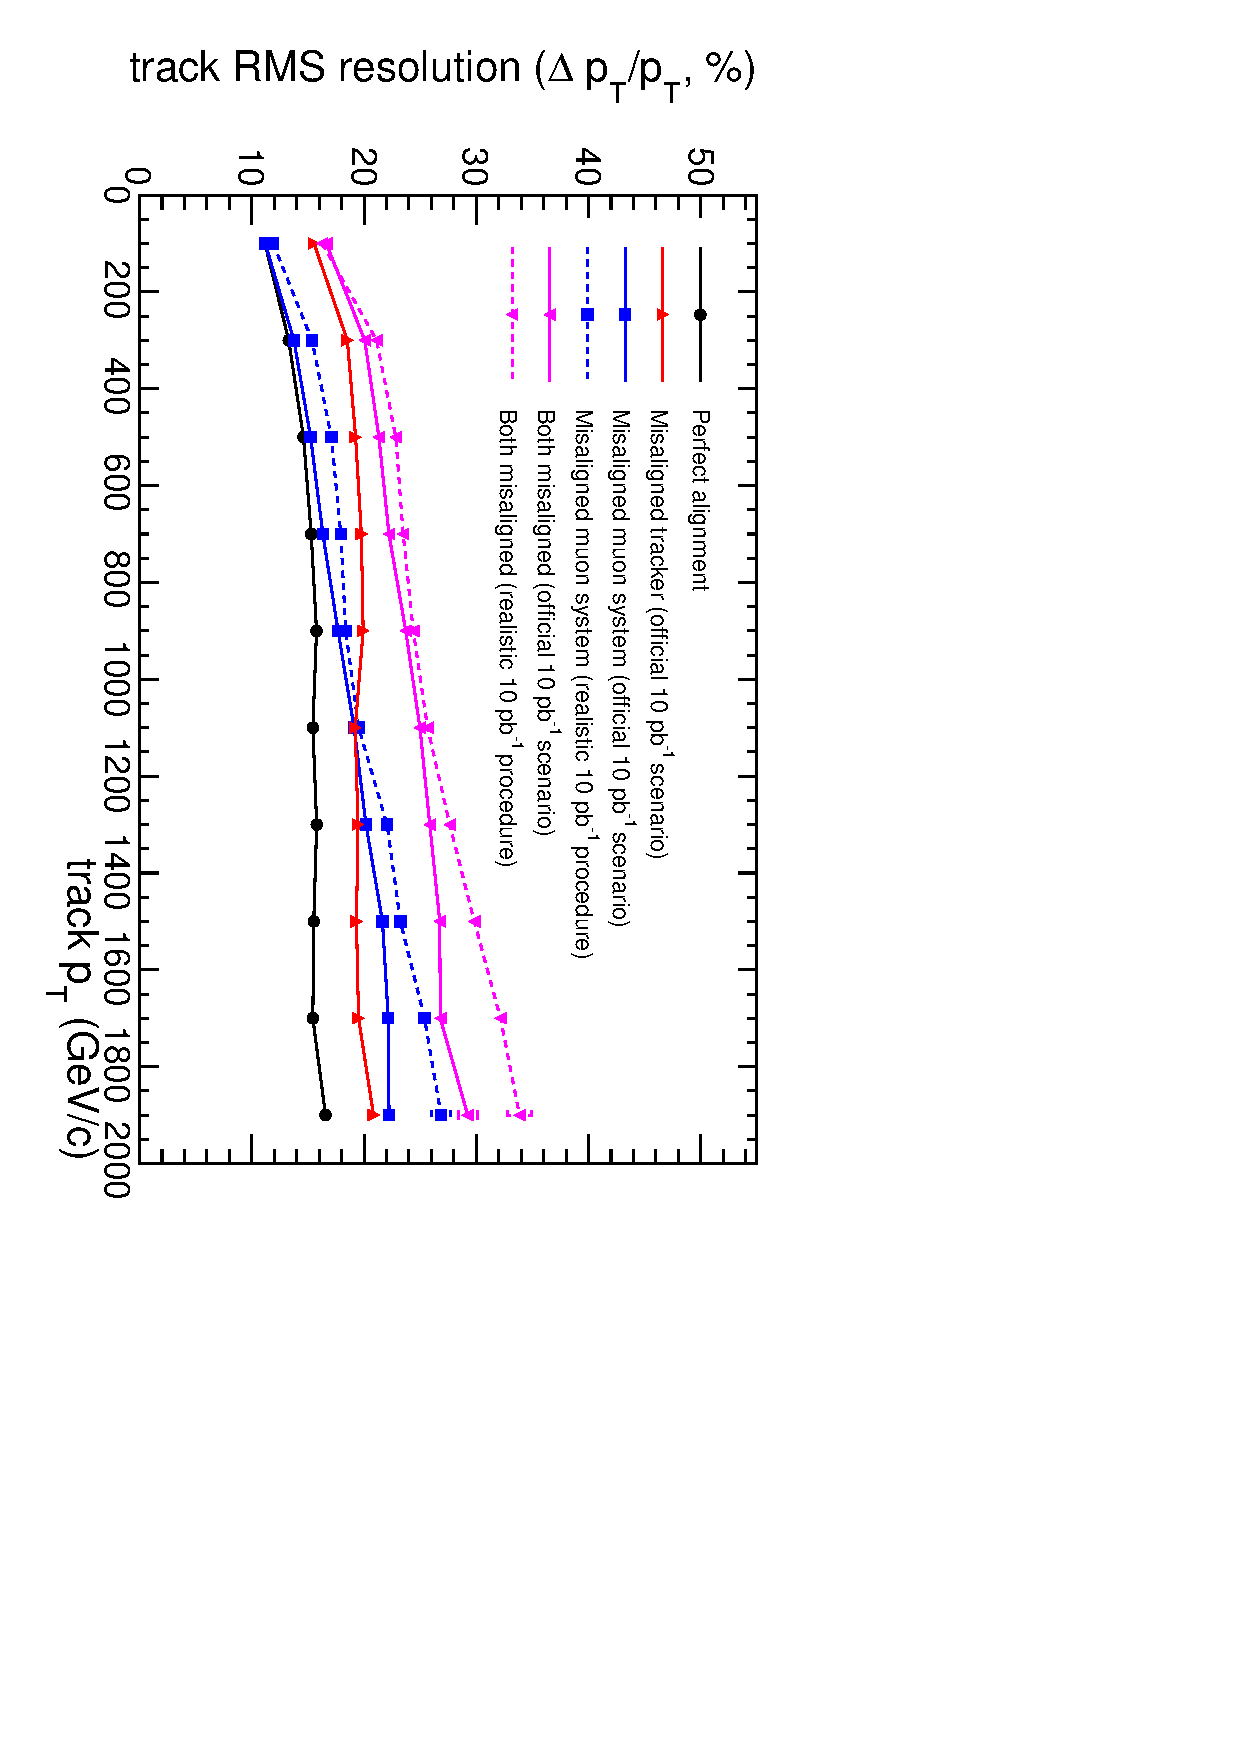
\includegraphics[height=\linewidth, angle=90]{ZSSM_Align_TrackRes_color.pdf}
\begin{itemize}
\item RMS of $\displaystyle \frac{\Delta p_T}{p_T}$ = RMS of $\displaystyle \frac{\Delta (1/p_T)}{(1/p_T)}$ (affected by tails)
\end{itemize}
\end{frame}

\section*{Summary}

\begin{frame}
\frametitle{Summary}
\begin{itemize}\setlength{\itemsep}{0.4 cm}
\item CSA07 unveiled a mistake that allowed ``MC-truth'' to leak into
our pre-November alignment results
\item Correcting that mistake, we observe that muon scattering is an
even more serious issue
\item We developed a procedure that addresses it, and are propagating
the new results
\item Results from new procedure match the official scenario; we are
working to improve them further
\item Quantified effects of tracker and new muon system misalignment
on TeV muons
\end{itemize}

\label{numpages}
\end{frame}

\section*{Backup slides}

\begin{frame}
\frametitle{Backup: sample points in the resolution plots}
\begin{itemize}
\item Worst-case: 3.5~TeV, both tracker and muon misaligned \\ (the rest are much more Gaussian)
\end{itemize}

\begin{center}
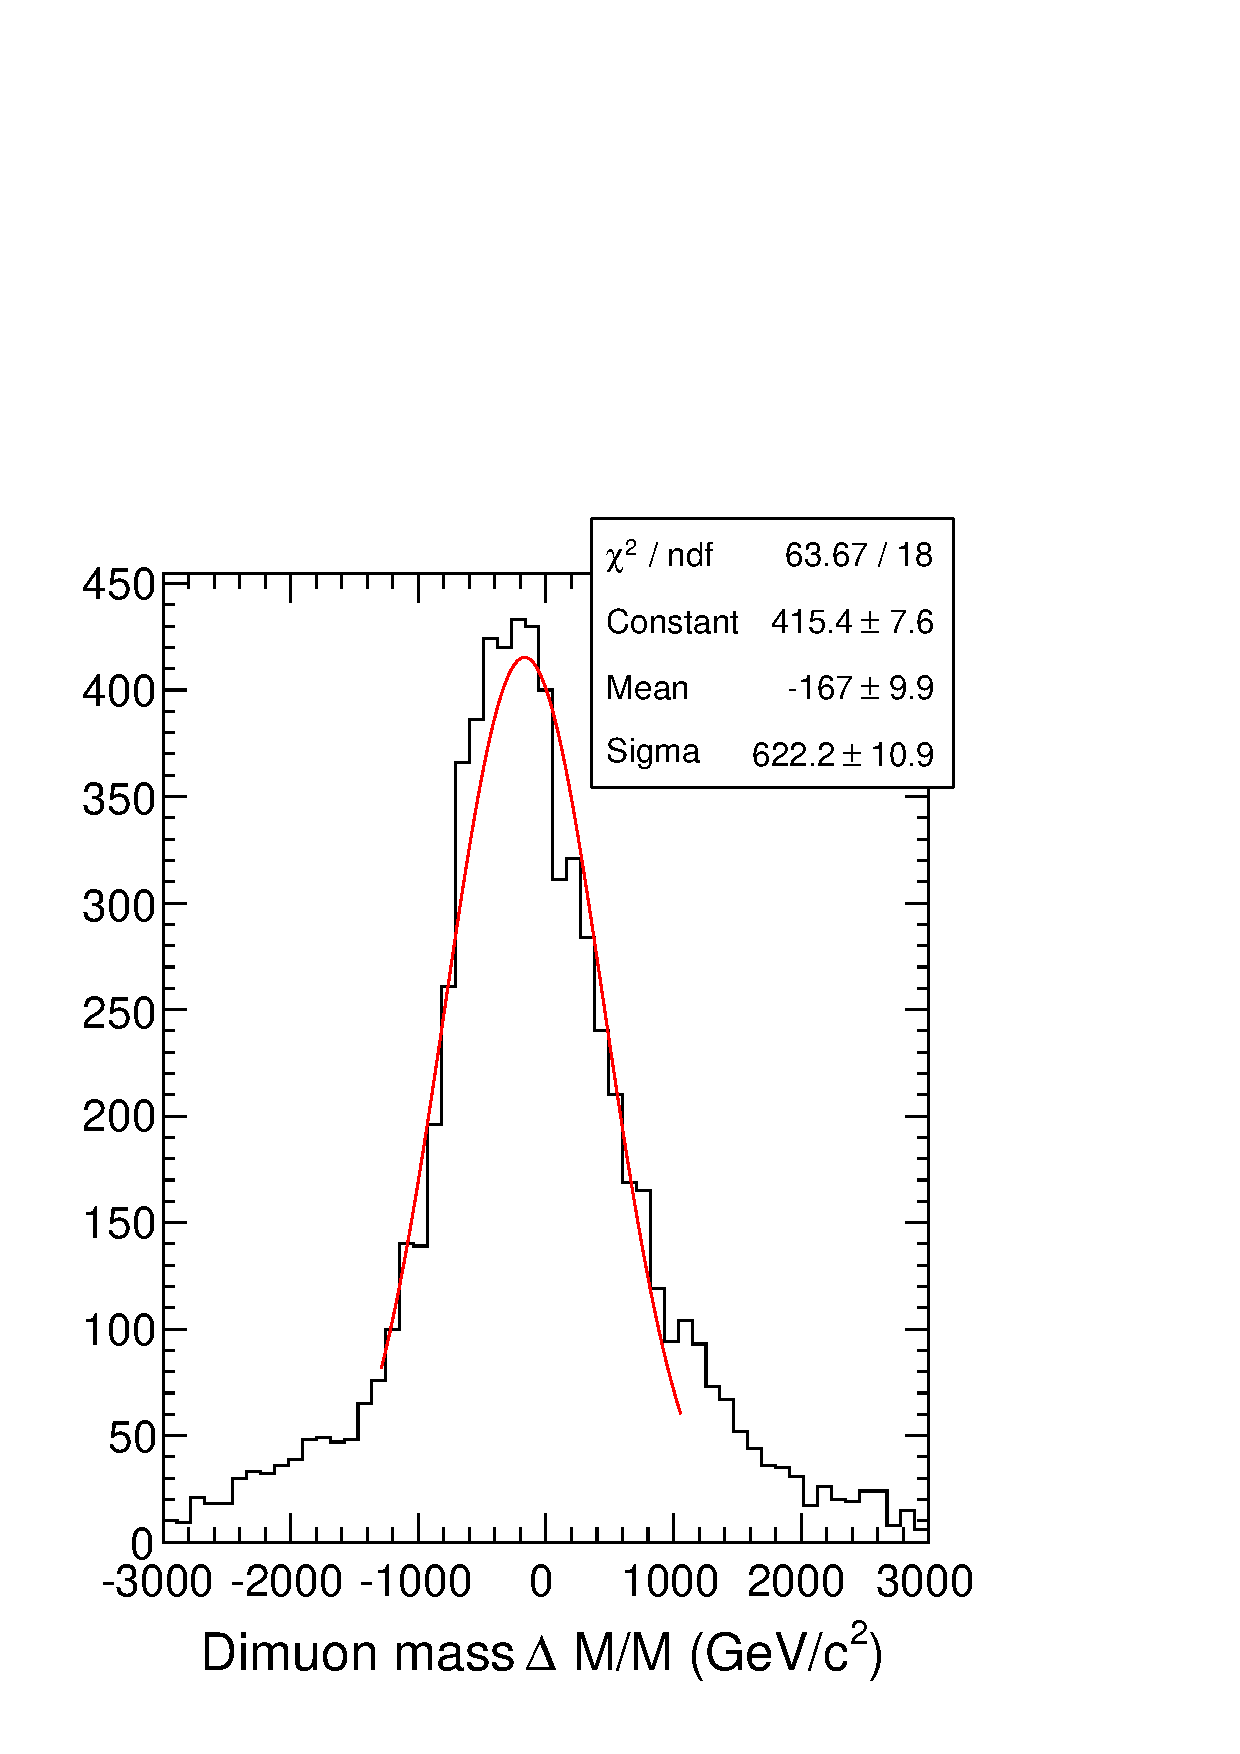
\includegraphics[width=0.38\linewidth]{sample_dimuon_peak_mybad.pdf}
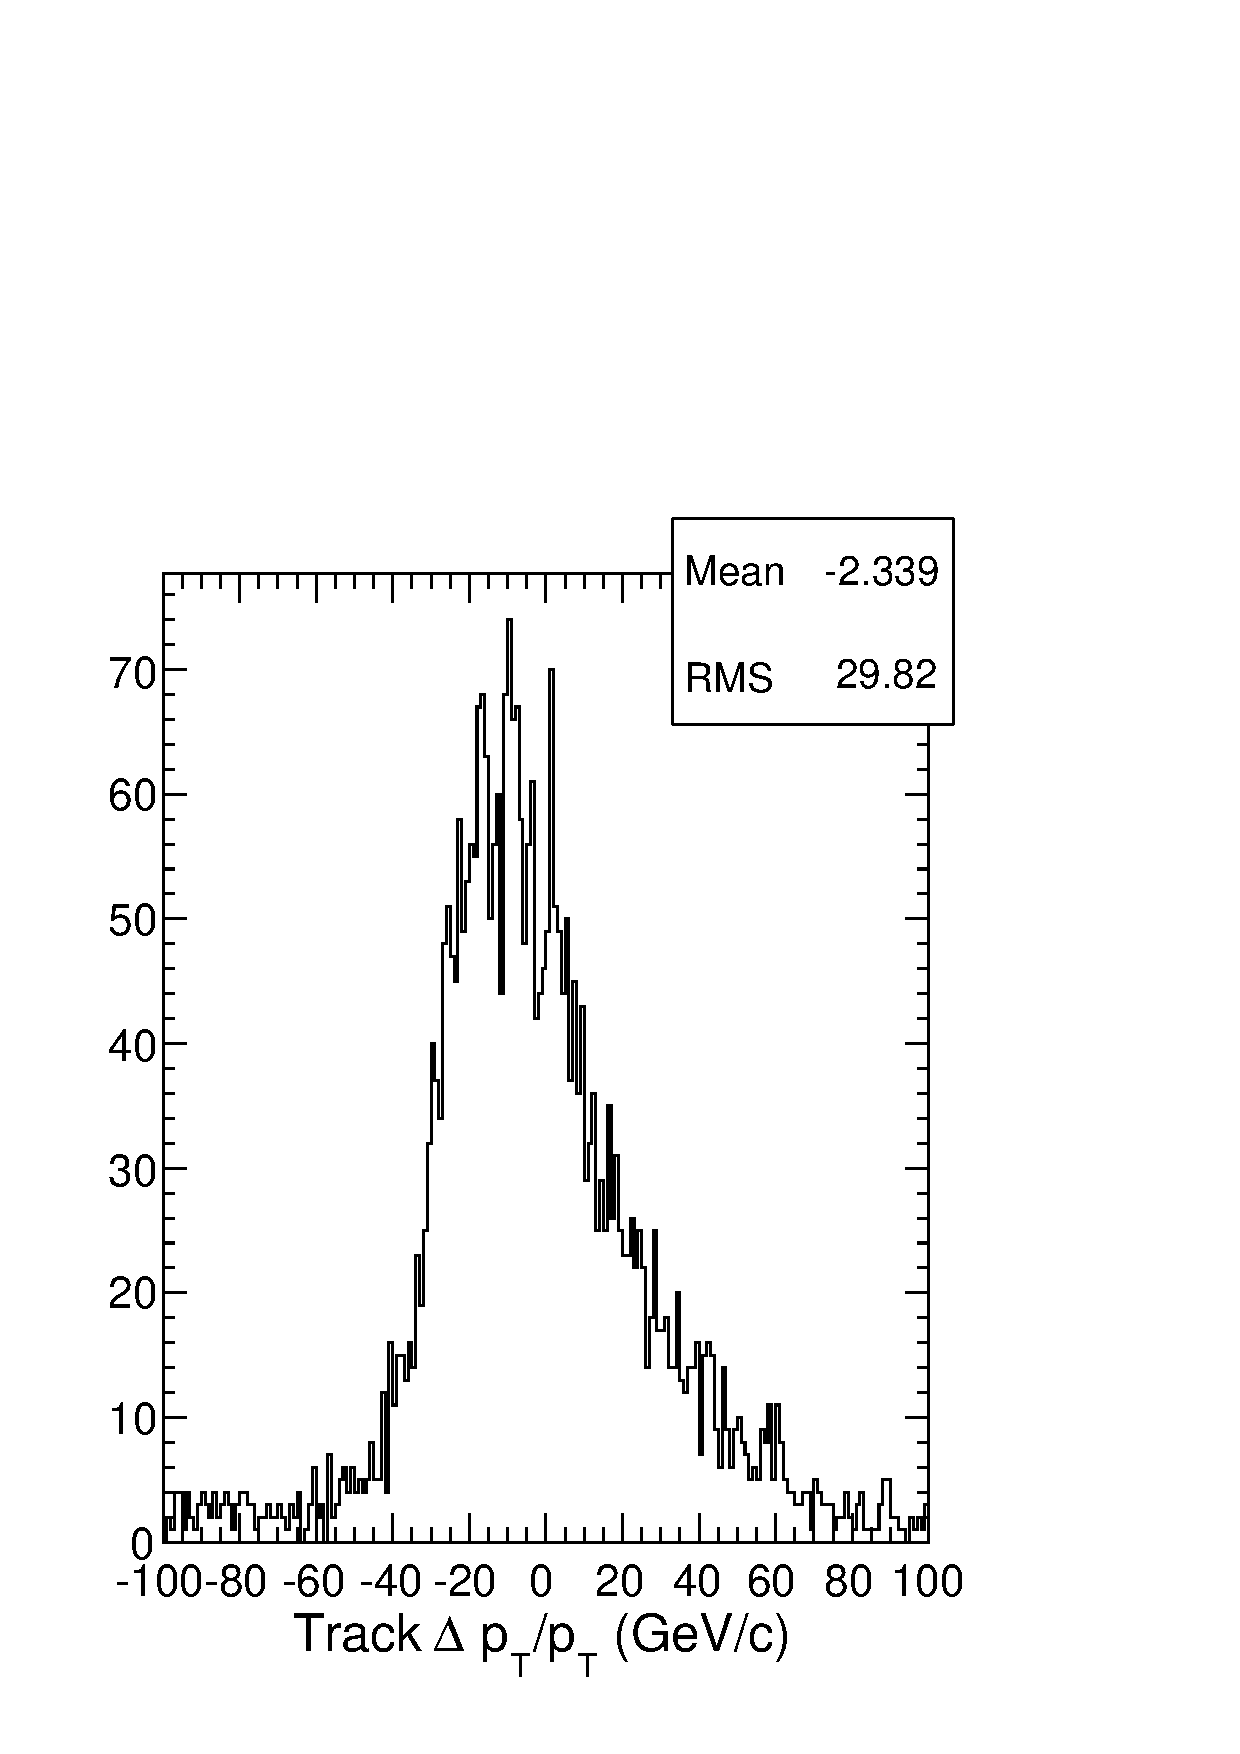
\includegraphics[width=0.38\linewidth]{sample_track_peak_mybad.pdf}
\end{center}

\vspace{-0.35 cm}
\begin{itemize}
\item Dimuon mass ``core resolution'' is a fit to $\pm$1.5$\sigma$
\item Track $p_T$ resolution is the RMS truncated at $\pm$100~GeV
\end{itemize}
\end{frame}


\end{document}
